\documentclass[10pt]{article}
\usepackage[utf8]{inputenc}
\usepackage[francais]{babel}
\usepackage{geometry}
\usepackage{graphicx}
\usepackage{fancyhdr}
\usepackage{hyperref}
\hypersetup{
    colorlinks,
    citecolor=black,
    filecolor=black,
    linkcolor=black,
    urlcolor=black
}

\geometry{hmargin=2cm, vmargin=2cm}

\def\blurb{Linköping University\\
IDA - The Department of Computer and Information Science}

\def\ligne#1{%
  \hbox to \hsize{%
    \vbox{\centering #1}}}%

\makeatletter
\def\maketitle{%
	\null
	\vfill
	\vbox{\centering \Large \textbf{\blurb}}
	\vspace{15mm}
	\vbox{\centering \LARGE \textbf{\@title}}
	\vspace{15mm}
	\vbox{\centering \@author}
	\vspace{8mm}
	\vbox{\centering \@date}
	\vfill
}

\title{TDDC17 - Lab 3 : Planning}
\author{Simon Vernhes \texttt{<simon@vernhes.eu>}}
\date{\today}

\begin{document}
  \pagestyle{fancyplain}
  \setlength{\parskip}{.6ex plus .4ex minus .4ex}
  \renewcommand{\headrulewidth}{0pt}
  \renewcommand{\footrulewidth}{0.6pt}
  \fancyhf{}
  \fancyhead{} 
  \lfoot{\@title \\ \@author}
  \rfoot{Page \thepage}
  \maketitle \clearpage
  
  \section{Introduction}
Early, computer graphic got the ambition the produce photo realistic images.

Ray tracing is a way to produce visual images. The main advantage of this technique among others is the photorealism of produced image.

To produce an image, a ray tracing engine trace the reverse path of the light, from the virtual eye (camera) through a virtual screen (the image) and calculate the color of visible objects. You can see an example on the figure \ref{img_intro}.

\begin{figure}[ht]
  \centering
  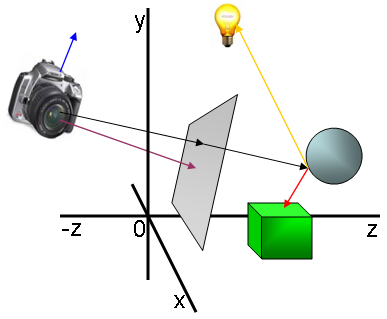
\includegraphics[height=7cm]{img/intro.png}
  \caption{Ray tracing}
  \label{img_intro}
\end{figure}

The eye (camera) look at a direction (purple arrow). A ray is traced through each pixel of the image (black arrow). The engine will try to find out where the ray intersect with an object (the sphere). The engine will find the color for this intersection by looking for the light and eventually reflexion of other objects (the cube).


  \section{Parameters}

We can easily increase the number of packages, numbers of cities, number of location within each city.


  \section{Investigation on different planners}

\subsection{Locations}

We will try to increase the number of locations.
The basic problem is composed of 4 cities with 4 truck, 1 train, 1 airplane. 2 airports (in city1 and city2) and 3 train station (city2, city3 and city4).

  \subsubsection{FF planer} \label{location_ff}

\begin{tabular}{|c|c|c|}
  \hline
  number of locations & total time & evaluated states (max depth) \\ \hline
  9  & 17.56s & 1823 (13) \\ \hline
  14 & 29.40s & 1823 (13) \\ \hline
  20 & 50.80s & 1823 (13) \\ \hline
\end{tabular}

This planer prefer to use truck to move a packet from a city to another instead of using faster transporter like train or airplane.

But as we can see, increasing the number of location don't increase the number of evaluated states, it only increase the time of searching. That means that it took more time to evaluate a state. This is understandable because at each state, if there is more location (even dummies one), more actions could be possibles. The planner have to compute action likes drive(truck location) for each locations.

For each entry, ff has returned the same plan. Which is the behavior we expected because the new locations are not in the goal.

  \subsubsection{IPP planer} \label{location_ipp}
\begin{tabular}{|c|c|c|}
  \hline
  number of locations & total time & actions tried \\ \hline
   9  & 5.72s  & 64345 \\ \hline
   14 & 57.33s & 363388 \\ \hline
   20 & 362.28s & 1067026 \\ \hline
\end{tabular}

Instead of FF planer, IPP choose to use both train and truck to move packet between cities.

IPP seams to take care of dummies locations. Maybe, it will try to bring packet to these locations to see if it can reach the goal that way.

Increasing the number of location seams to increase polynomially the number of explored states, and so increase polynomially the total time of exploration.

However, IPP seams to reach a first goal node extremely quickly.


\subsection{Cities}

Now we will try to increase the number en cities. And so, we also must increase the number of location. One office and one airport per city. The basic problem is the same as before, with 4 objects to move.

  \subsubsection{FF planer}

\begin{tabular}{|c|c|c|}
  \hline
  number of cities & total time & evaluated states (max depth) \\ \hline
  4  & 6.14s & 1823 (13) \\ \hline
  10 & 22.95s & 1823 (13) \\ \hline
  15 & 50.44s & 1823 (13) \\ \hline
\end{tabular}

Same remarks. See previously section \ref{location_ff}

  \subsubsection{IPP planer}

\begin{tabular}{|c|c|c|}
  \hline
  number of locations & total time & actions tried \\ \hline
   4  & 5.67s & 64345 \\ \hline
   10 & 47.62s & 116623 \\ \hline
   15 & 162.86s & 200943 \\ \hline
\end{tabular}

Same remarks. See previously section \ref{location_ipp}


\subsection{Packages}

Now we will try to increase the number of packages. All packages will not necessarily be in the goal (don't need to be moved).

  \subsubsection{FF planer}

\begin{tabular}{|c|c|c|}
  \hline
  total packages (in goal) & total time & evaluated states (max depth) \\ \hline
  4 (4)  & 5.96s & 1823 (13) \\ \hline
  5 (4)  & 380.95s & 1823 (13) \\ \hline
  5 (5)  & 282.43s & 1565 (13) \\ \hline
  6 (6)  & X & X \\ \hline
  8 (4)  & X & X \\ \hline
  8 (8)  & X & X \\ \hline
\end{tabular}

FF planner doesn't explore more node if there's more dummy packet (packet which doesn't have to be moved). However it spend more time evaluating each node (compare line 1 and 2).

  \subsubsection{IPP planer}

\begin{tabular}{|c|c|c|}
  \hline
  total packages (in goal) & total time & actions tried \\ \hline
  4 (4)  & 5.72s  & 64345 \\ \hline
  5 (4)  & 6.41s & 64345 \\ \hline
  5 (5)  & 22.95s & 237012 \\ \hline
  6 (6)  & 351.24s  & 4062129 \\ \hline
  8 (4)  & 8.34s & 64345 \\ \hline
  8 (8)  & X & X \\ \hline
\end{tabular}

As we can see, IPP don't care about packet which are not is the goal.

However, increasing packages in goal increase greatly the number of actions tried and so the total time.





  \section{Conclusion}

All these experiments showed that FF planner always explored the same number of states if we add dummies objects (like new cities, locations or packet which are not involved in the goal). But spend more time evaluating each node, evaluating with these dummies objects.

Unlike FF planer, IPP take cares about these dummies and try more actions when there's more dummies objects. But IPP planner seems to be able to handle more packet when FF planner is not.


\end{document}

